\chapter{Algoritmo ottimizzato tramite decomposizioni bilanciate}
\label{cap:3}
In questo capitolo viene presentata un'ottimizzazione all'algoritmo descritto nel capitolo \ref{TODO_riferimento_al_capitolo}. %TODO non si ottimizza il problema ma l'algoritmo!
basata sull'idea di decomporre gli alberi $T$ in una coppia di alberi $T'$ e $T''$ con un numero simile di nodi.
Si fa vedere, inoltre, come modificare i dettagli implementativi precedentemente discussi.

\section{Decomposizioni bilanciate di un albero}
\label{cap:3 par:1}
Nel precedente capitolo, dato un albero $ T $ con $|T|=k$, viene considerata la decomposizione di $T$ in due alberi $ T' $ e $ T''$. 
Dipendentemente da $T$, tale decomposizione può restituire un albero $T'$ (o $T''$) contenente un numero esiguo di nodi rispetto a $|T|$.
Un esempio dove questo fenomeno è particolarmente evidente si verifica quando $T$ è una stella di $k$ nodi per cui $|T'|=k-1$ e $|T''|=1$.

In questa sezione si mostrerà che dato un albero $T$ \`e sempre possibile ricavare una decomposizione ``bilanciata'' dell'albero  in due alberi $ T' $ e $ T'' $ le cui cardinalit\`a distino al al più di una costante moltiplicativa.

Prima di poter enunciare e dimostrare il risultato principale occorre dare delle nozioni preliminari.

\newtheorem{definizione}{Definizione}[section]

\begin{definizione}
	\label{definizioneDeco} 
Sia $T_r$ un albero, con $k$ nodi, radicato nel nodo $r$.
Diremo che la coppia $(A,B)$, dove  $A$ e $B$ sono due sottoalberi di $T_r$, \`e una decomposizione per l'albero $ T_r $ se:
\begin{itemize}
	\item $| A | + | B | = k$; e
	\item $A \cap B = \{r\}$. %TODO A e B sono alberi. Cosa vuol dire A \cap B?
\end{itemize}
\end{definizione}


\begin{definizione}
\label{lemmaDeco}
Data una funzione $f : \mathbb{N} \to \mathbb{N}$ ed un albero $ T $ con $ k $, diremo che $ (A,B) $ \`e una decomposizione $ f(k) $-bilanciata se:
\begin{equation*}
	\max{ \{|A| , |B| \} }  \le  f(k).
\end{equation*}
\end{definizione}



%TODO Aggiungi una frase di raccordo dicendo che per il seguito faremo uso della nozione di centroide di un albero, definita di seguito.

\begin{definizione}
Per ogni nodo $ v $ di un albero $ T $, le diramazioni di $ T $  rispetto a $ v $, sono tutti i sottoalberi massimali di $ T $ non contenenti $ v $. 
Per ogni $ v \in T $, si definisce $\alpha(v)$ come il massimo numero di nodi tra le diramazioni rispetto a $ v $.\\ %TODO cambiato diramazioni "di" $v$ -> diramazione **rispetto** a $v$, in accordo con la definizione appena data
Un nodo $ v $ di un albero $ T $ con $ n $ nodi, \`e un nodo centroide se $\alpha(v)\le\frac{n}{2}$.
\end{definizione}

Il centroide di un albero non \`e necessariamente unico, infatti Jordan \cite{jordan1869assemblages}  ha dimostrato che, dato un albero $ T $ con $ n $ nodi:
\begin{enumerate}
	\renewcommand{\labelenumi}{\roman{enumi}}
	\item $ T $ ha un singolo centroide $ v $ e $\alpha(v) < \frac{n}{2}$, oppure
	\item$ T $ ha due nodi centroidi (adiacenti) $v_1$ e $v_2$ tali che $\alpha(v_1) = \alpha(v_2) = \frac{n}{2}$, in questo caso il numero di nodi $ n $ \`e pari.
\end{enumerate}

Esistono diversi algoritmi per la ricerca del centroide, quello utilizzato in questa tesi \`e un algoritmo con complessit\`a temporale lineare nel numero di nodi che fa uso di una visita in profondità (DFS) dell'albero. \\
Il primo passo da effettuare \`e calcolare i valori $\alpha(v)$ per ogni nodo $ v$ dell'albero $T$.\\
Innanzitutto per ogni nodo $v$ di $T $ indichiamo con $ \eta(v) $ il numero di nodi presenti nel sottoalbero radicato in $ v $ di $ T $.
A questo punto si radica $T$ in un nodo arbitrario e si procede ad una visita DFS dell'albero, memorizzando, per ogni $v$, il rispettivo valore $ \eta(v) $, che può essere calcolato ricorsivamente nel seguente modo 
\begin{equation}
\label{eq:eta_centroide}
\eta(v) = 1 + \sum_{\substack{u \ figlio \ di \ v \ in \ T} } { \eta(u)}.
\end{equation}

Si noti che, nel caso particolare in cui $v$ è una foglia, la formula precedente implica che $\eta(v)=1$.
Una volta conclusa la visita, si pu\`o determinare $ \alpha(v) $ per ogni nodo $ v $ in $ T $, come segue
\[ \alpha(v) = \max\{ \max_{\substack{u \ figlio \ di \ v \ in \ T}} {\eta(u)} \ , \ |T| - \eta(v) \}. \]
\noindent Una volta calcolato il valore di $ \alpha(v) $ per ogni $  v \in T $ si verifica per quali valori  risulta $\alpha(v)\le\frac{|T|}{2}$.\\
%Nel caso ci fosse un unico nodo $ v $ che soddisfa la precedente condizione, come in (i),  allora tale nodo rappresenta l'unico  centroide dell'albero $ T $.
%Nel caso, invece, ce ne fossero due, come in (ii), per esempio $ v_1 $ e $ v_2 $,  l'albero $ T $ conterr\`a due centroidi, rispettivamente $ v_1 $ e $ v_2 $.\\
Per verificare che l'algoritmo ha una complessit\`a $ T(n) $ lineare sul numero di nodi.
Basta notare che la visita DFS su un albero $ T $ di $ n $ nodi richiede un tempo $ O(n) $ per essere completata.
%
%A questa quantit\`a va sommato il tempo necessario per determinare per ogni nodo $ v $ di $ T $ il rispettivo grado, che indichiamo con $ \delta(v) $, anche questo richiede un tempo lineare sul numero di nodi $ n $. %TODO ??????
%
A questa quantità va sommato il tempo necessario per calcolare, per ogni nodo $v$ di $T$, la quantità $\eta(v)$ usando la formula \eqref{eq:eta_centroide}. Ciò richede tempo $O(1 + \delta(v))$ dove $\delta(v)$ indica il grado di $v$ in $T$.

In particolare insieme quanto detto finora, ed usando l'identità $\sum_{v} \delta(v) = 2(n-1)$, quello che si ottiene \`e:
\[  T(n) = O(n + \sum_{v}(1+\delta(v)))= O(n + n + \sum_{v}\delta(v)) = O(n+n+2n-2)=O(n).
\] 

Nell'esempio \ref{es1} si pu\`o vedere l'applicazione dell'algoritmo per la ricerca del centroide.
	\begin{figure}[htbp]
		\centering
		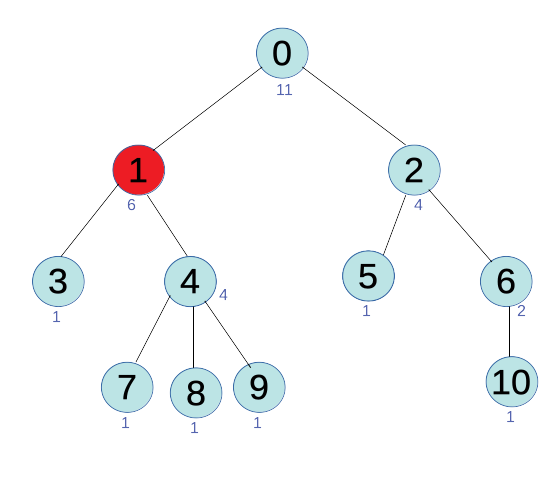
\includegraphics[width=5cm]{capitolo3/grafo2}
		\caption{Albero $ T $  per la ricerca del centroide} 
		\label{fig:2}
\end{figure}

\newtheorem{esempio}[definizione]{Esempio}
\begin{esempio}
	\label{es1}
Si consideri l'albero T in figura \ref{fig:2} per la ricerca del nodo centroide.
Per ogni nodo $ v $ di $ T $ numerato da 0 a 10,  viene calcolato $\alpha(v)$ . \\
Quello che si ottiene \`e: %TODO Non è chiaro come questo esempio stia aiutando... forse puoi almeno far vedere i valori di \eta ?
\begin{center}
	\centering
	\begin{tabular}{ c c c c c  }
		$\alpha(0) = 6$ & & $\alpha(1) = 7$ & & $\alpha(2) = 5$ \\ 
		$\alpha(3) = 9$ && $\alpha(4) = 10$ &&  $\alpha(5) =  7$ \\  
		$\alpha(6) = 10$ && $\alpha(7) = 10$ && $\alpha(8) = 10$ \\
		$\alpha(9) = 10$ && $\alpha(10) = 10$ &&
	\end{tabular}
\end{center}

Poich\'e $ \left\lfloor\frac{n}{2} \right\rfloor = \left\lfloor \frac{11}{2} \right\rfloor = 5$, l'unico nodo per cui la disuguaglianza, $\alpha(v)\le\frac{n}{2}$, risulta vera \`e il nodo 2, infatti $5\le 5$.\\
Poich\`e il numero di nodi \`e dispari certamente questo sar\`a l'unico centroide dell'albero T (figura \ref{fig:2}). 
\demo
\end{esempio}\mbox{}\\

L'ultimo punto da considerare prima di poter enunciare e dimostrare il risultato principale di questa sezione riguarda la definizione di un algoritmo valido per decomporre due insiemi di nodi, %TODO Sei sicura che quello che vogliamo decomporre siano *due insiemi di nodi*?
che chiameremo $ T' $ e $ T'' $, in maniera $ f(k) $-bilanciata.\\
Siano dati in input un albero $ T $, con $ k\ge 3 $ nodi, ed un fattore di bilanciamento definito da una funzione $ f(k) $. %TODO A cosa ti seve il fattore di bilanciamento IN INPUT?
Si suppone inoltre, senza perdita di generalit\`a, che i sottoalberi radicati nei figli della radice $ r $ di $ T $ siano ordinati in ordine non crescente.
Da questo deriva che, supponendo che $ r $ abbia $ \ell $ figli, vi saranno $ \ell $ alberi radicati tali che: $ |T_{i}|\ge |T_{i+1}|  \forall {i = 1,\dots, \ell-1} $, inoltre si indica con $ S $ la seguente quantit\`a $ S=\sum_{i=1}^{\ell}|T_i| $.
Sia $i = \max \{ j : \sum_{h=1}^{j} |T_h| \le \frac{2 S}{3} \}$. L'algoritmo selezionerà $T'$ come il sottoalbero di $T$ indotto da $r$ e dai nodi in $T_1, \dots, T_i$, e $T''$ di conseguenza.
La decomposizione di $T$ in $T'$ e $T''$ restituita dall'algoritmo appena descritto, il cui pseudocodice è mostrato in TODO, è $ (\lfloor \frac{2}{3}(k-1) \rfloor + 1)$-bilanciata, come dimostrato dal seguente teorema.

	\begin{figure}[htbp]
	\centering
	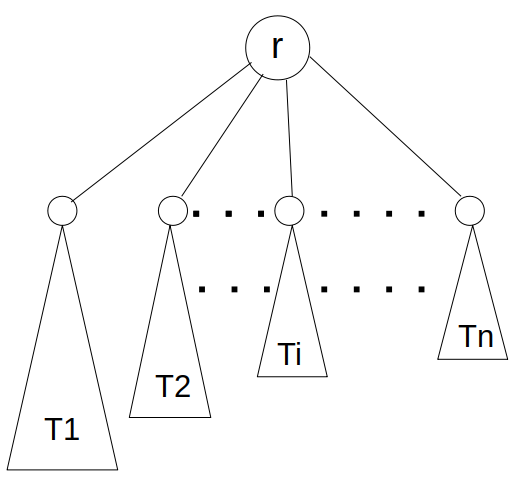
\includegraphics[width=5cm]{capitolo3/grafo3}
	\caption{Esempio di albero $ T $ radicato in $ r $, con $ k $ nodi, valido come input per l'algoritmo \ref{algoritmo1}} 
	\label{fig:3} %TODO Aggiungi una figura in cui fai vedere la decomposizione risultante. Puoi fissare un albero specifico ai fini dell'esempio.
	%TODO I nomi degli alberi in figura sono sbagliati. I numeri dovrebbero essere a pedice
\end{figure}

\begin{algorithm}[H]
	\label{algoritmo1}
	\SetAlgoLined
	\caption{Algoritmo per il calcolo di una decomposizione $ (\lfloor \frac{2}{3}(k-1) \rfloor + 1)$-bilanciata di un albero $T$ }
	\textbf{input} : Albero $ T $ con $ k $ nodi\;
	$r \gets $ un centroide di $T$\;
	$T_r \gets $ albero $T$ radicato in $r$\;
	$\ell \gets$ grado di $r$ in $T$\; 
	Sia $ |T_i| $ l'albero radicato nell'$ i $-esimo figlio di $ r $.\;
	%TODO Devi supporre che $|T_i| \ge |T_{i+1}|$ per $i=1, \dots, \ell-1$
	$ S \gets \sum_{i=1}^{n}|T_i| $;\\
	\For{$ i = 1,\dots,\ell $}
	{
		\If{$ \sum_{j=1}^{i}{|T_j|} > \frac{2}{3}\cdot S $}
		{
			$ T'\gets $ sottoalbero di  di $ T_r $ indotto da $ \{r\} \cup \bigcup_{j=1}^{i-1}V(T_j)$;\\ %TODO Hai definito la notazione V(T)??
			$ T'' \gets $ sottoalbero di $ T_r $ indotto da $ V(T) \setminus T'$;\\ %TODO Cosa vuol dire sottrarre un albero da un insieme di nodi?
			\textbf{return} ($ T',T'' $);\\
		}	 
}
\end{algorithm}

%Una volta concluso l'algoritmo \ref{algoritmo1} si avr\`a una coppia $ (T',T'') $ tale che : $ \max (|T'|,|T''|) \le f(k) $. %TODO: Ma cosa è questo f(k)???



\newtheorem{teorema1}[definizione]{Teorema}
\begin{teorema1}
	\label{teorema1 cap3 sez1}
Per ogni albero T di $k \ge 3$ nodi esiste un nodo $r$ di T  tale che l'albero $T_r$, ottenuto radicando $T$ in $r$, ammette una decomposizione $ (\lfloor \frac{2}{3}(k-1) \rfloor + 1)$-bilanciata. Inoltre tale decomposizione $ (T',T'')$ soddisfa $ |T'| \ge 2+\frac{(k-1)}{3} $.
\end{teorema1}
\begin{proof}
	Sia $r$ sia un centroide dell'albero $ T $ e $T_r$ l'albero $ T $ radicato in $ r $ \\  	Inoltre, si suppone che i sottoalberi radicati nei figli di $r$ siano ordinati in maniera non crescente rispetto al loro numero di nodi. %TODO aggiunto "rispetto al loro numero di nodi". Non è chiaro come due sottoalberi andrebbero confrontanti per poter essere ordinati altrimenti
	Si applichi a $ T_r $ l'algoritmo \ref{algoritmo1} precedentemente descritto. Sia $ \{T_i \ | \  i=1,\dots,n\} $ l'insieme dei sottoalberi radicati negli $\ell$ figli di $ r $ e si consideri il primo valore di $ i $ tale che la condizione dell'\texttt{if} di riga $ 6 $ nell'algoritmo \ref{algoritmo1} risulti vera (si noti che tale valore di $ i $ esiste sempre dal momento che per $ i = \ell $ la condizione \`e verificata).
	Sia 
	\[ S = \sum_{j=1}^{n}{|T_i|} = (k-1 ) \]\\
	e sia
	\[ x = \sum_{j=1}^{i-1}{|T_j|} \]\\
	Distinguiamo due casi
	\begin{itemize}
	\item $i \ge 3$. In questo caso si ha che
	\begin{equation}\label{1}
		x+|T_i| > \frac{2}{3}\cdot S
	\end{equation}
	Inoltre per l'ordine in cui i sottoalberi $ T_i $ sono considerati
	\begin{equation}\label{2}
	|T_i| \le \frac{S}{i} \le \frac{S}{3}	.
	\end{equation}
	Sottraendo la disequazione \eqref{2} alla \eqref{1} si ottiene che 
	\begin{equation}\label{3}
	x > \frac{2}{3}\cdot S - \frac{S}{3} = \frac{S}{3}.
	\end{equation}
 	\item $ \textbf{i=2} $ Anche in questo caso come nel precedente vale la disequazione \eqref{1}.\\
 	Inoltre, essendo $ i = 2 $, per l'ordine in cui vengono considerati gli alberi $T_i$ si pu\`o dire che
 	\begin{equation}\label{4}
 	x = |T_1| \ge |T_2| = |T_i|
 	\end{equation}
 	Pertanto, sfruttando la disequazione \eqref{4} combinata con la \eqref{1} si ha che
 	\begin{equation}\label{5}
 	2x > \frac{2}{3} \cdot S \Rightarrow x > \frac{S}{3}
 	\end{equation}
	\end{itemize}
Per entrambi i casi otteniamo che 
\[ x > \frac{S}{3} \]
Dal momento che $ x $ \`e intero otteniamo 
\[ x \ge \left\lfloor \frac{S}{3}\right\rfloor  + 1\]
Pertanto si avr\`a che 
\begin{equation}\label{6}
	\left\lfloor \frac{S}{3}\right\rfloor  + 1 \le x \le \left\lfloor \frac{2}{3}\cdot S \right\rfloor
\end{equation} 
dove $  x \le \left\lfloor \frac{2}{3}\cdot S \right\rfloor $ \`e banalmente verificata per la scelta di $ i $.
Quindi 
\begin{equation}\label{7}
|T'| = 1+x \le 1 + \left\lfloor \frac{2}{3}\cdot S \right\rfloor = 1 + \left\lfloor \frac{2}{3} \cdot (k-1) \right\rfloor	
\end{equation}
e
\begin{equation}\label{8}
|T''| = 1 + S - x = 1+S-1 - \left\lfloor \frac{S}{3}\right\rfloor = \left\lceil \frac{2}{3}\cdot S \right\rceil = \left\lceil \frac{2}{3} \cdot (k-1) \right\rceil 	
\end{equation}
Poich\`e
\[1 + \left\lfloor \frac{2}{3} \cdot (k-1) \right\rfloor \ge \left\lceil \frac{2}{3} \cdot (k-1) \right\rceil \] 
Possiamo concludere che
\[ \max\{|T'|,|T''|\} \le 1 + \left\lfloor \frac{2}{3} \cdot (k-1) \right\rfloor \]
Infine da \eqref{6} segue che
\[ 
|T'| = 1+ x \ge 1+ (1 +  \left\lfloor \frac{S}{3}\right\rfloor ) = 2 +  \left\lfloor \frac{(k-1)}{3}\right\rfloor
\]
\end{proof}
 
 	
\section{Algoritmo}
\label{cap:3 par:2}
In questa sezione si vede come \`e stato utilizzato il risultato della sezione \ref{cap:3 par:1} per ottimizzare e migliorare l'algoritmo \ref{algoritmo} descritto nel capitolo \ref{cap 2} (paragrafo \ref{section1}).\\
Quello che si faceva in precedenza era, dato un albero $ T_C $, con $ T $ un albero radicato di $ k $ nodi i cui colori giacciono in $ C $, si procedeva al conteggio delle occorrenze di $ T_C $ nel seguente modo
\[	
c(T_c,v)=\frac{1}{\beta_T}\sum_{(u,v)\in E} \;\; \sum_{\substack{C', C'' \subset C : |C'| = |T'| \\C' \cup C'' = C  \\ C' \cap C'' = \emptyset}}c(T'_{C'},v)\cdot c(T''_{C''},u) 
\]
dove  $T'$ e $T''$ sono due alberi ottenuti tramite un'opportuna decomposizione di $T$  tali che $|T'|, |T''| \in \{1, \dots, k-1\}$, $ T'' $ (e $|T''| = k - |T'|$), mentre $ T'_ {C'} = (T', C') $ e $ T''_{C''} = (T'', C'') $ sono due treelet colorati, radicati rispettivamente in $ v $ ed $ u $.

In questa nuova versione, invece, $ T_C $ viene suddiviso in due alberi $ T' $ e $ T'' $ tali da  rispettare il principio delle decomposizioni bilanciate e pi\`u nello specifico il teorema \ref{teorema1 cap3 sez1}.\\
Innanzitutto si determina se l'albero $ T_C $ \`e radicato in uno dei centroidi, nel caso in cui ci\`o non fosse vero, l'albero $ T_c $ non viene conteggiato.
Successivamente viene suddiviso $ T_C $ in due alberi $ T'_{C'} $ e $ T''_{C''} $ tali che: entrambi gli alberi risultino radicati nella stessa radice $ r $ di $ T $,  $ \max\{|T'|,|T''|\} \le 1 + \left\lfloor \frac{2}{3} \cdot (k-1) \right\rfloor $ e $ |T'| \ge 2+\left\lfloor\frac{k-1}{3} \right\rfloor $.
Inoltre i due insiemi $ C' $ e $ C'' $ dovranno essere tali che $C' \cup C'' = C$ e $ C' \cap C'' = \{c_r\} $, dove $ c_r $ il colore del nodo radice.\\
Come nel caso precedente, l'algoritmo che si utilizza per il conteggio delle occorrenze dei $ k $-treelet colorati in $ G $ utilizza la tecnica della programmazione dinamica, quindi si procede dai sottoproblemi pi\`u piccoli arrivando a quello pi\`u grande.\\
Anche qui per ogni nodo $ v $ si inizializza $ c(T_{C_0} , v) = 1 $, dove $T_{C_0} = (T, C_0)$, $T$ \`e il treelet di $1$ nodo e $ C_0 = \{c_v\} $.
Questa volta, per\`o, per calcolare le occorrenze dei $ k $-treelet radicati in ogni $ v \in V $ di $ G $ non sar\`a necessario aver calcolato il numero di  occorrenze degli $h$-treelet con $h=1,\dots,k-1 $, ma sar\`a necessario calcolarli solo fino a $h \le  \left\lfloor \frac{2}{3}(k-1)\right\rfloor +1 $.
Tale conteggio verr\`a eseguito sulla base dell'algoritmo \ref{algoritmo} di sezione \ref{section1}. \\
Per calcolare per ogni nodo $v \in V  $ di $ G $ il numero $ c(T_C,v) $ di occorrenze dei $ k $-treelet (non indotti) radicati in $ v $ isomorfi a $ T $ i cui colori giacciono nell'insieme $ C $ si sfrutta la seguente relazione:
\[
c(T_C,v) = \frac{1}{\gamma_T}\sum_{\substack{
C',C'' \subseteq C : |C'| = |T'| \\
C' \cup C'' = C \\ 
C' \cap C'' = \{c_r\}}}
c(T'_{C'},v)\cdot c(T''_{C''},v)
 \] 
con $\gamma_T$ la nuova costante di normalizzazione che \`e uguale a $ \binom{p}{q} $, dove $ p  $ \`e il numero di sottoalberi di $ T $ isomorfi al sottoalbero radicato nell'ultimo figlio della radice di $ T' $ e $ q $ il numero di sottoalberi radicati a partire dal primo figlio della radice di $ T'' $ isomorfi al sottoalbero radicato nell'ultimo figlio della radice di $ T' $.
Di seguito viene riportato lo pseudocodice dell'algoritmo precedentemente descritto.

\begin{algorithm}[H]
	\label{algoritmo2}
	\SetAlgoLined
	\caption{TODO}
	\textbf{input} : Grafo $ G =(V,E) $, dimensione deI treelet di interesse $ k \ge 3 $;\\		
	\For{$ h = 1$ to $ \left\lfloor \frac{2}{3}(k-1) \right\rfloor +1 $}{
	Si calcolano le occorrenze secondo quanto riportato nell'Algoritmo \ref{algoritmo};\\
	}

	\For{$ v \in V $}{
	\ForEach{$ T : |T| = k $}{
		Sia $ c $ un centroide di $ T $\;
		\If{$ c \ != \ v $} {\textbf{break}; } %TODO: Break? Sei sicura? Sicura sicura?
		Suddivido $ T $ in due alberi $ T' $ e $ T'' $ come descritto in precedenza\; %Metti un riferimneto
			\[c(T_C,v) = \frac{1}{\gamma_T}\sum_{\substack{
C',C'' \subseteq C : |C'| = |T'| \\
C' \cup C'' = C \\ 
C' \cap C'' = \{c_r\}}}
c(T'_{C'},v)\cdot c(T''_{C''},v)\]
	}	
} 	
\end{algorithm}\bigskip

Come nell'algortimo \ref{algoritmo} il numero di occorrenze di $ T $ è calcolato con un approccio basato sulla scomposizione dell'albero in due sottoalberi,  per\`o, anche in questo caso nella tesi l'algoritmo \ref{algoritmo2} \'e stato implementato nel verso opposto, ossia a partire dai conteggi di due sottoalberi $ T' $ e $ T'' $ si \`e ottenuto i conteggi relativi a $ T $. %TODO Non si capisce: è sempre vero che i conteggi di T si ottengono da quelli di T' e T''
Perci\`o per calcolare le occorrenze dei $ k $-treelet in $ G $, $ \forall v \in V $ di $ G $ si prendono tutte le possibili coppie di alberi colorati $ (T'_{C'}, T''_{C''} )$ radicate in $ v $ tali che: $ 2+ \left\lfloor \frac{(k-1)}{3}  \right\rfloor \le |T'| \le \left\lfloor \frac{2}{3}(k-1) \right\rfloor  +1 $ e $ |T''| = k-|T'| $.
Prima di poterle unire nell'albero $ T_C $ è necessario 
verificare che la decomposizione bilanciata di $T$ calcolata dall'algoritmo [TODO RIF all'algoritmo di decomposizione] concida con $T'$ e $T''$. In particolare, se $r$ è la radice di $T'$ e $T''$:
\begin{itemize}
	\label{prova}
	\item bisogna verificare che la coppia $ (T',T'') $ sia una decomposizione bilanciata per $ T $.
	Pertanto dovr\`a risultare che $ |T'| - 1 \le \left\lfloor\frac{2}{3}(k-1)\right\rfloor $ e che aggiungendo a tale quantit\`a la cardinalit\`a del sottoalbero radicato nel primo figlio di $ T'' $, denotata con $ t'' $, si abbia che $ |T'| + t'' - 1 \ge \left\lfloor\frac{2}{3}(k-1)\right\rfloor $.
	\item Anche in questo caso bisogner\`a garantire l'ordinamento sulla struttura dell'albero. %TODO Di nuovo: l'ordinamento non ha solo a che vedere con la dimensione. Questo punto è sbagliato.
	Pertanto non sar\`a possibile unire $ T' $ e $ T'' $ se la dimensione del sottoalbero radicato nell'ultimo figlio della radice di $ T' $ \`e minore del sottoalbero radicato nel primo figlio della radice di $ T'' $.
	\item Bisogna garantire che sia rispettato i vincoli sui colori: $C' \cup C'' = C$ e $ C' \cap C'' = \{c_r\}$, ossia i due insiemi $C'$ e $C''$ condividono esclusivamente in colore della radice $ r $.
	\item bisogna verificare che il nodo $ r $ sia il centroide dell'albero $ T $ risultante dall'unione di $ T' $ e $ T'' $. 
\end{itemize}
Queste condizioni sono necessarie affinch\`e l'unione %TODO Come prime, non hai parlato di unioni finora
tra gli alberi $ T'_{C'} $ e $ T''_{C''} $ produca un albero valido $ T_C $.

Come si nota, anche in questo caso, i conteggi inizialmente vengono fatti su ogni $ v \in V $, ma poich\`e in questa tesi interessano le occorrenze dei diversi $ k $-treelet in $ G $  sar\'a necessario aggregare gli alberi radicati su ogni $ v $ di $ G $, unendoli a seconda della propria struttura e sommando le rispettive occorrenze.

Nel caso in cui si abbiano due centroidi, la scelta su quale radicare l'albero  \`e deterministica. %TODO Veramente da quanto descritto sopra stai vedendo l'albero due volte. L'idea di preferire uno dei due centroidi è un trucco per assicurarsi che (alcuni) degli alberi con 2 centroidi vengano contati 1 sola volta.
Nel caso in cui gli alberi ottenuti radicando $ T $ in ognuno di essi abbiano strutture differenti, viene scelto quello che tra i due ha una struttura pi\`u piccola.
Altrimenti se gli alberi ottenuti sono identici, viene scelto uno dei due in maniera arbitraria.  %TODO Questa frase è proprio falsa...


Questo implica che tali alberi vengano conteggiati un numero di volte doppio rispetto al conteggio reale. %TODO Veramente se la frase precedente fosse vera implicherebbe esattamente il contrario... se ogni albero è conteggiato in un centroide scelto in maniera arbitraria allora i conteggi sono giusti!
Perci\`o in fase di normalizzazione i conteggi di tutti gli alberi per cui questa condizione risulta vera saranno ulteriormente divisi per due.

%TODO Ricorda al lettore che questi conteggi si riferiscono al numero di occorrenze con colori distinti e che per ottenere uno stimatore unbiased del numero N(T) di occorrenze di T bisogna moltiplicare per k^k / k!. 
%Guarda la descrizione corrispondente del capitolo precedente

\section{Dettagli implementativi. Modifica e aggiunte alle rappresentazioni}
\label{cap 3:3}
Anche in questa nuova versione gli oggetti principali manipolati restano i treelet colorati e le occorrenze associate.

Ogni treelet colorato $ T_C = (T,C)$ continua ad avere una rappresentazione unica, memorizzata usando interi a 64 bit.
I bit hanno lo stesso ordinamento della precedente versione.
Quello che cambia, per\`o, \`e la suddivisione dei bit:
\begin{itemize}
	\item i bit da 0-3 contengono un valore numerico che \`e pari ad 1 se l'albero ha un solo centroide o due centroidi tali che, gli alberi ottenuti radicando $ T $ in ognuno di essi risultino diversi.
	Mentre \`e pari a  2 se l'albero ha due centroidi tali che, gli alberi ottenuti radicando $ T $ in ognuno di essi risultino uguali.
	\item  i bit da 4-7 contengono il numero $\mu$ di sottoalberi in $ T'' $ radicati a partire dal primo figlio della radice isomorfi al sottoalbero radicato nell'ultimo figlio della radice di $ T' $.
	\item i bit da 8-11 contengono il valore $ q $ necessario nel calcolo binomiale $ \binom{p}{q} $ usato in fase di normalizzazione.
	La somma di $ q $ con $\mu$ restituisce $ p $.
	\item i bit da 12-63 restano invariati alla versione precedente.	  
\end{itemize} 

La struttura dell'albero \`e codificata esattamente come la versione precedente,in particolare i sottoalberi radicati nei figli della radice dell'albero, appaiono in ordine non crescente rispetto alle relative rappresentazioni, definendo implicitamente un ordinamento totale sui treelet (colorati).\\\\
Alle precedenti operazioni sugli alberi se ne aggiungono delle nuove che sono:
\begin{itemize}
	\item $ \textbf{balance\_merge}(T',T'') $ : fa l'unione di due alberi $ T' $ e $ T'' $ in maniera bilanciata.
	All'interno del metodo viene garantito che tutte le condizioni necessarie affinch\`e l'unione avvenga, descritte in fondo al paragrafo precedente, siano verificate.
	\item $ \textbf{normalization\_factor\_balanced}(T) $ : restituisce il fattore di normalizzazione $ \gamma_T $ dell'unione bilanciata.
\end{itemize}\mbox{}\\
Un'altra differenza rispetto la versione precedente riguarda la costruzione della tabelle.
Infatti, seguendo quanto descritto in algoritmo \ref{algoritmo2}, verranno costruite tutte le entrate da 1 a  $ \left\lfloor \frac{2}{3}(k-1) \right\rfloor +1 $ come veniva fatto nella versione precedente.
Mentre non verranno costruite le $ h $ tabelle tali che: $ \left\lfloor \frac{2}{3}(k-1) \right\rfloor +1 < h < k $, ma si proceder\`a direttamente alla costruzione della tabella contenente i $ k $-treelet.\\
Anche in questa versione i treelet colorati raggiunti $ \forall v \in V $ verranno aggregati e i loro conteggi sommati ed anche in questa versione i conteggi di nodi differenti  (per ogni valore di $ h $ fissato) vengono calcolati in parallelo da pi\`u thread.